\section{TOCL+ Tool Support and Implementation}

\subsection{Support tool architecture}

\begin{figure}
    \centering
    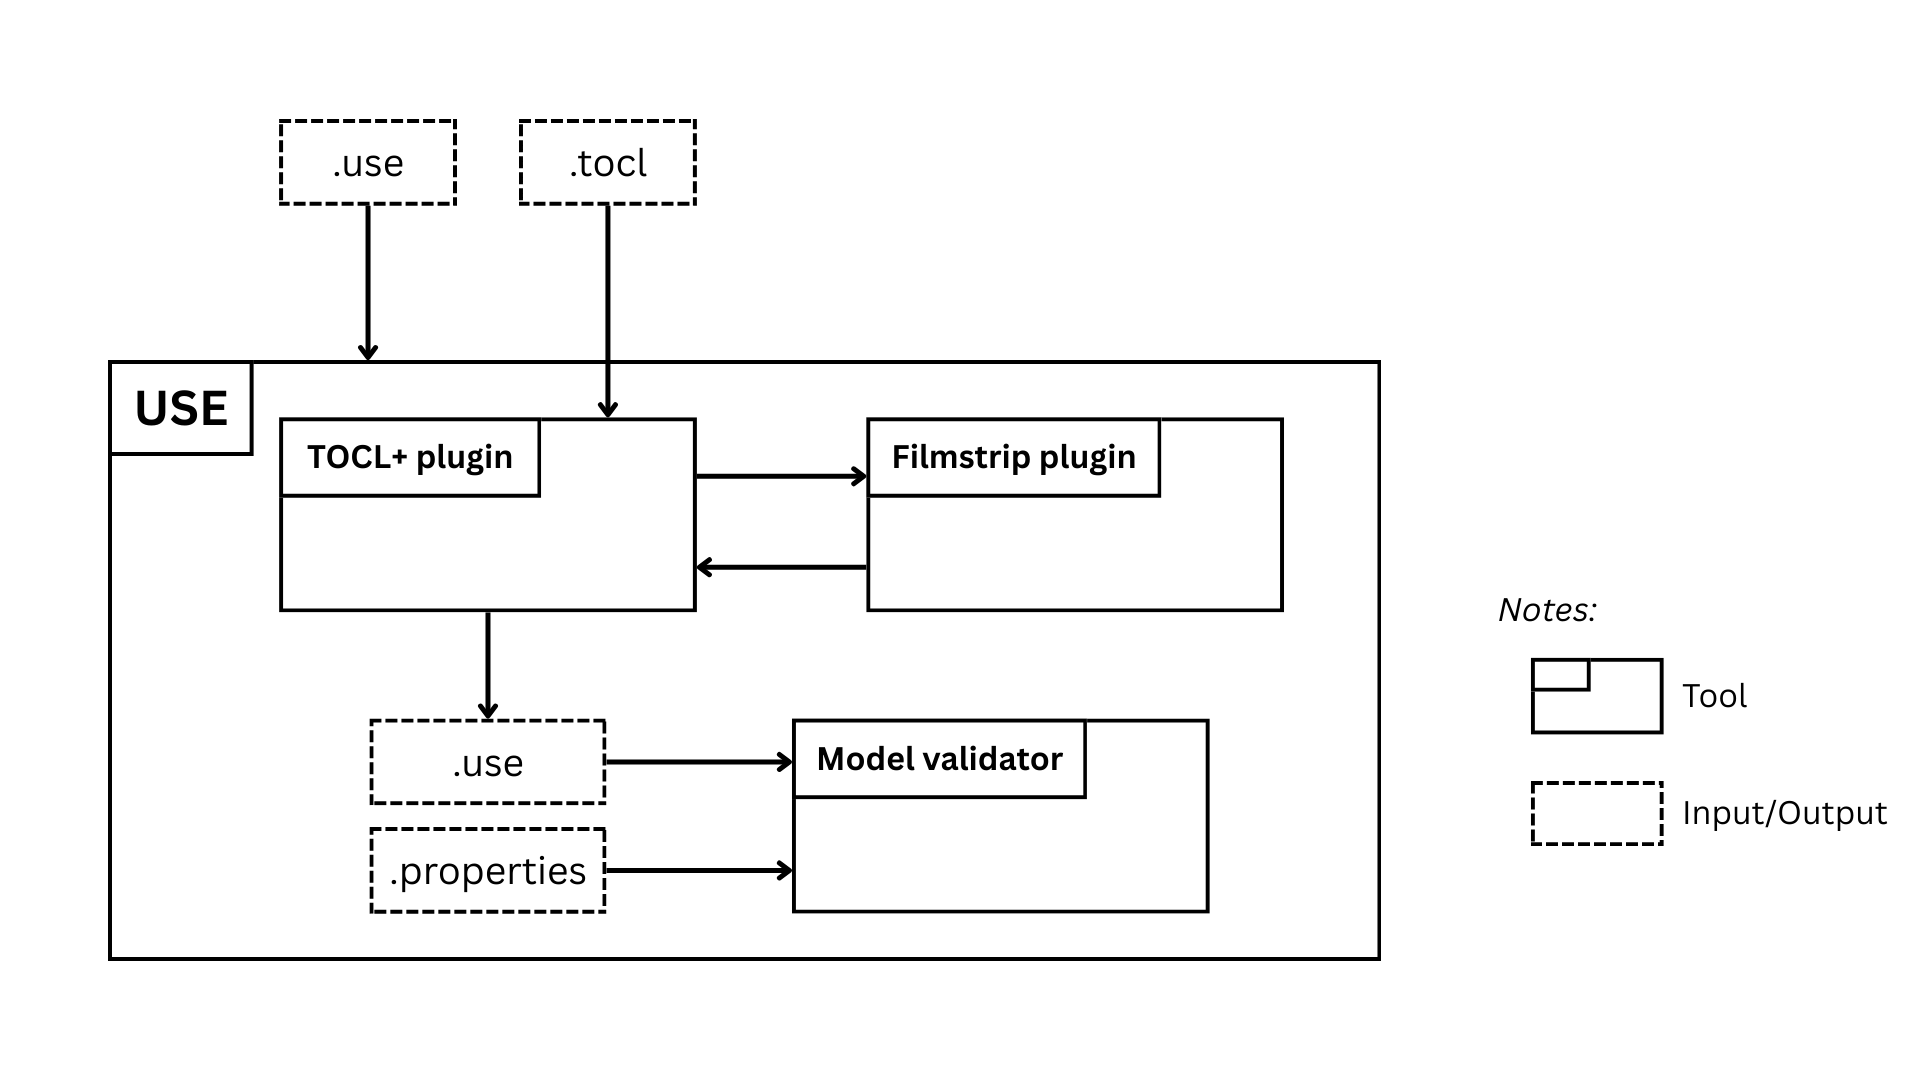
\includegraphics[width=1\textwidth]{figures/c3/Architecture_overview.png}
    \caption{Support Tool Architecture and Verification Workflow.}
    \label{sec:plugin_support_tool_architecture}
\end{figure}

\hspace{1cm} Figure \ref{sec:plugin_support_tool_architecture} illustrates the architecture and workflow of our TOCL+ support tool. This integrated verification framework combines several components: the existing USE environment, the Filmstrip plugin, our TOCL+ plugin, and the Model Validator. The architecture maintains a clear separation between modeling, specification, and verification concerns while providing a cohesive workflow for users.

The verification process consists of five distinct steps, beginning with preparation and ending with validation. First, the user prepares two input files: a standard \texttt{.use} file containing the UML/OCL application model and a \texttt{.tocl} file containing TOCL+ property specifications. Second, the user loads the application model into USE to make it available for transformation. Third, the user activates our plugin through the USE interface, selecting both a destination path for the output model and the \texttt{.tocl} file containing the temporal properties to verify.

Internally, the plugin then executes a two-phase transformation process. In the first phase, it invokes the Filmstrip plugin to transform the application model into a filmstrip model following the rules described in Section~\ref{subsec:filmstripping}. In the second phase, it processes the TOCL+ expressions using our ANTLR4-generated parser and listener components, which implement the transformation rules for converting temporal specifications into equivalent OCL constraints. These generated constraints are added to the list of invariants in the output model file alongside the filmstrip model elements.

To complete the verification process, the user loads this output model back into USE together with a configuration file that establishes search bounds, and then employs the Model Validator to analyze the constraints. The validator systematically explores the search space, determining whether the temporal properties are satisfied and providing a model instance as evidence when applicable.

Our primary contribution in this architecture is the TOCL+ plugin, specifically the TOCL+ to OCL transformation component that enables the verification of temporal properties using existing OCL tools. The implementation details of this transformation process, including the translation rules for different temporal operators and event constructs, are presented in the next subsection.


\subsection{Implementation of TOCL+ to OCL Transformation}

\hspace{1cm} The core of our contribution lies in the transformation of TOCL+ 
expressions into equivalent OCL constraints that can be verified over filmstrip 
models. This transformation process involves systematically mapping temporal operators 
and event constructs to structural navigations through snapshots and operation calls. 
In this section, we describe our implementation approach and the key translation 
patterns we developed.

Our transformation approach is inspired by the work of \cite{TOCL2OCL}, who 
transformed TOCL \cite{TOCL} into OCL in the context of a Snapshot-Transition Model 
(STM). While their approach also converts temporal properties into static ones, we 
adapted and extended it to work within the filmstrip model context, particularly 
addressing the challenges of representing events and maintaining object identity 
across snapshots.

We implemented the transformation using ANTLR4, a parser generator that creates a 
parse tree from TOCL+ expressions. The transformation process employs listener 
components that traverse this parse tree and produce corresponding OCL expressions 
by overriding the generated listener methods. As the parser walks through each node 
in the parse tree, our listeners apply the appropriate translation rules, constructing 
equivalent OCL constraints that navigate through the filmstrip structure.

For the transformation to work correctly, we needed to establish fundamental 
navigation operations that allow constraints to traverse the filmstrip model. 
The key operations include: \texttt{self.snapshot} to get the snapshot associated 
with an object in the current state; \texttt{snapshot.pred()} and 
\texttt{snapshot.succ()} to navigate to the previous and next snapshots; and 
\texttt{object.pred} and \texttt{object.succ} to navigate to the corresponding 
object in the previous and next states.

A significant challenge in the filmstrip approach is maintaining object identity 
across different snapshots. While the filmstrip model provides \texttt{pred} and 
\texttt{succ} associations to navigate between objects in adjacent snapshots, it 
doesn't inherently provide a mechanism to identify the same conceptual object across 
non-adjacent states. To address this limitation, we require modelers to add an 
\texttt{id} attribute to all classes in the application model. As seen in Figure 
\ref{fig:object_diagram_liveness}, this allows us to identify the same logical 
object (e.g., three Application objects with id 0) across different snapshots. 
Our plugin adds additional constraints to ensure this id remains consistent 
throughout the timeline, enabling reliable temporal navigation.

Table \ref{tab:TOCL2OCL} presents the complete set of translation patterns we developed for TOCL+ operators and event constructs. Each pattern systematically maps a TOCL+ construct to an equivalent OCL expression interpreted over the filmstrip model. The patterns use placeholders (indicated by square brackets) that get substituted during the transformation process: \texttt{[s |= P]} indicates that property P holds in snapshot s; \texttt{[ContextSnapshot]} is the snapshot in which the property is evaluated; \texttt{[ContextObject]} is the object on which the property is evaluated; and \texttt{[OpClassName]} is the class representing an operation call in the filmstrip model.

For example, the translation of the temporal operator \texttt{sometime P} (pattern 5) uses the closure operation to navigate through all future snapshots, checking if property P holds in at least one of them. Similarly, the \texttt{becomesTrue(P)} event construct (pattern 13) compares the evaluation of P between the current snapshot and its predecessor.

Listing \ref{lst:becomesTrue_translation} demonstrates how we implemented the translation for the \texttt{becomesTrue} event construct. The implementation extracts the boolean expression to be evaluated, identifies the current context, and constructs OCL expressions that compare the property's evaluation in adjacent snapshots. The critical part of this implementation is how it handles object identity through the \texttt{id} attribute:

%%% Sample
% Using ANTLR4 listeners, we implemented the transformation as Java code built on 
% the TOCL parser we created. The listeners traverse the parse tree of a TOCL+
% expression and produce the corresponding OCL expression. The transformation from TOCL to OCL is implemented by overriding generated listener methods of the
% ANTLR4 TOCLparser. To use these rules we walk the parse tree generated by the TOCL parser.
% The above implementation is inspired by \cite{TOCL2OCL}, in their work, they 
% transformed TOCL \cite{TOCL} into OCL in the context of a STM which is another kind
% of class model to represent dynamic properties in the form of static properties. We 
% adopted their approach and applied it in our approach which transform TOCL+ to OCL 
% within the context of filmtrip model.

% To transform TOCL+ expressions, we defined translations for TOCL operators and events
% to OCL, as shown in Table \ref{tab:TOCL2OCL}. To create these translations, 
% we utilized some query operations. The self.snapshot query gets the snapshot
% associated with an object in the "current state" or the state where the expression 
% is being evaluated. The pred() and succ() operations when applied to a snapshot get 
% the snapshot in the previous and next state, respectively. For objects to navigate
% to the corresponding object in the next and previous state, we use the two associations
% .succ and .pred. Note that the parts of the patterns that are between square brackets
% (e.g. [s |= P], [ContextSnapshot], [ContextObject]) must be replaced when instances 
% of the patterns are specified. The expression [s |= P] in the OCL patterns mean that 
% the property P holds in the snapshot s. P is a boolean expression in the context of 
% a class, for example C. When using the patterns to write temporal properties, the OCL 
% expression representing s |= P is generated by navigating from the snapshot s to C,
% the context of OCL expression P. The [ContextSnapshot] and [ContextObject] will be 
% replaced with the corresponding snapshot and object when the model is transformed. 
% For example, in the translation of the liveness property shown in Listing
% \ref{lst:ocl_liveness} the [ContextSnapshot] is replaced with the local vairable s
% inside the exists query. 
% Note that the use id attribute. Recall from Fig. \ref{fig:object_diagram_liveness},
% there are three Application objects with id 0 and three with id 1. Because filmstrip 
% model does not provide any means to identify the same object across different states, 
% it only provides the pred and succ associations to navigate between them. In order to 
% overcome the above drawback of filmstrip model, the modeler must add id attribute to all the 
% application model classes. And internally when TOCL+ plugin transforms the model
% we add additional constraints to make sure the id stays consistent between different 
% states. And the id attribute is put into use in the OCL translation for 

% After defining these translations, we created rules for them using listeners. These 
% rules take the OCL translation of each TOCL operator and simply replace the 
% appropriate parts with the children of the corresponding parse tree node.
% For instance, when translating a becomesTrue event, we extract the boolean expression
% and construct the corresponding OCL expression to be evaluated. We do this using
% getOCL(ParseTree ctx) operation, which gets the text associated with node ctx. In 
% addition, we also keep track of the original TOCL+ expression in the variable
% originalEvent. After the translation, we push both the translated event expression
% and the original event expression into a stack, which will be popped at the end of 
% traversing the entire parse tree. Listing \ref{lst:becomesTrue_translation} shows 
% an example of the implementation of the becomesTrue event using an ANTLR4 listener.


\begin{lstlisting}[
    style=javastyle,
    caption={Translation of becomesTrue event to OCL.},
    label={lst:becomesTrue_translation}
]
TokenStream tokens = parser.getTokenStream();
String originalEvent = tokens.getText(ctx);
String translatedEvent;
// P
String expressionToSatisfy = getOCL(ctx.getChild(2)); 
// e.g., "system", "application"
String roleName = toLowerFirstChar(currentContext); 
String currentSnapshot = "self.snapshot"; 
String selectObject = "->any(o | o.id = self.id)";

// e.g. self.snapshot.system->any(o | o.id = self.id)
String objectAtCurrentSnapshot = currentSnapshot + "." + roleName + selectObject;
String objectAtPreviousSnapshot = currentSnapshot + ".pred()." + roleName + selectObject;
String P_at_currentSnapshot = expressionToSatisfy.replace("self", "currentObject");
String P_at_previousSnapshot = expressionToSatisfy.replace("self", "previousObject");

translatedEvent = 
"let currentObject = " + objectAtCurrentSnapshot +
" in let previousObject = " + objectAtPreviousSnapshot +
" in not (" + P_at_previousSnapshot + ") and (" + P_at_currentSnapshot + ")";

eventStack.push(translatedEvent);
eventStack.push(originalEvent);    
\end{lstlisting}

\begin{table}[htbp]
\caption{Translation of TOCL+ operators and events to OCL.}
\label{tab:TOCL2OCL}
\begin{tabularx}{\textwidth}{|>{\footnotesize}p{0.6cm}|>{\scriptsize\raggedright\arraybackslash}p{4cm}|>{\scriptsize\raggedright\arraybackslash}X|}
    \hline
    \textbf{No.} & \textbf{TOCL+} & \textbf{OCL Translation} \\
    \hline
    1 & 
    next P &
    let nextSnapshot:Snapshot = self.snapshot.succ() in [nextSnapshot |= P] \\
    \hline
    2 &
    always P &
    let CS:Snapshot = self.snapshot in Set\{CS\}->closure(s | s.succ())->forAll(s | [s |= P]) \\
    \hline  
    3 &
    always P until Q &
    let CS:Snapshot = self.snapshot
    in let FS:Set(Snapshot) = Set\{CS.succ()\}->closure(s | s.succ())
    in let AllFSQ:Set(Snapshot) = FS->select(s | [s |= Q])
    in let FSQ:Snapshot = AllFSQ->any(s | Set\{s\}->closure(s | s.succ())->includesAll(AllFSQ))
    in let afterQ:Set(Snapshot) = Set\{FSQ\}->closure(s | s.succ())
    in let FSP:Set(Snapshot) = FS->select(s | [s |= P])
    in if FSQ.isDefined() then (if (FSP->size() > 0) then (FS-afterQ = FSP-afterQ) else false endif) else (FS = FSP) endif \\
    \hline
    4 &
    always P since Q &
    let CS:Snapshot = self.snapshot
    in let PS:Set(Snapshot) = Set\{CS.pred()\}->closure(s | s.pred())
    in let AllPSQ:Set(Snapshot) = PS->select(s | [s |= Q])
    in let PSQ:Snapshot = AllPSQ->any(s | Set\{s\}->closure(s | s.pred())->includesAll(AllPSQ))
    in let beforeQ:Set(Snapshot) = Set\{PSQ\}->closure(s | s.pred())
    in let PSP:Set(Snapshot) = PS->including(CS)->select(s | [s |= P])
    in if PSQ.isDefined() then (if (PSP->size() > 0) then (PS->including(CS)-beforeQ = PSP-beforeQ) else false endif) else (PSP = PS->including(CS)) endif \\
    \hline
    5 &
    sometime P &
    let CS:Snapshot = self.snapshot in Set\{CS\}->closure(s | s.succ())->exists(s | [s |= P]) \\
    \hline
    6 &
    sometime P before Q &
    let FS:Set(Snapshot) = Set\{self.snapshot\}->closure(s | s.succ())
    in let PreS:Set(Snapshot) = Set\{self.snapshot.pred()\}->closure(s | s.pred())
    in let AllFSQ:Set(Snapshot) = FS->select(s | [s |= Q])
    in let FSQ:Snapshot = AllFSQ->any(s | Set\{s\}->closure(s | s.succ())->includesAll(AllFSQ))
    in let FSP:Set(Snapshot) = FS->select(s | [s |= P])
    in if FSQ.isDefined() then (if (FSP->size() > 0) then ((Set\{FSQ.pred()\}->closure(s | s.pred())-PreS)->exists(s\_1 | FSP->includes(s\_1))) else false endif) else false endif \\
    \hline
    7 &
    sometime P since Q &
    let CS:Snapshot = self.snapshot
    in let PS:Set(Snapshot) = Set\{CS.pred()\}->closure(s | s.pred())
    in let AllPSQ:Set(Snapshot) = PS->select(s | [s |= Q])
    in let PSQ:Snapshot = AllPSQ->any(s | Set\{s\}->closure(s | s.pred())->includesAll(AllPSQ))
    in let PSP:Set(Snapshot) = PS->select(s | [s |= P])
    in if PSQ.isDefined() then (Set{PSQ}->closure(s | s.succ())->excluding(null)->intersection(PS)->exists(s | PSP->includes(s))) else false endif \\ 
    \hline
    8 &
    previous P &
    let previousSnapshot:Snapshot = self.snapshot.pred() in [previousSnapshot |= P] \\
    \hline
    9 &
    sometimePast P &
    let CS:Snapshot = self.snapshot in Set\{CS.pred()\}->closure(s | s.pred())->exists(s | [s |= P]) \\
    \hline
    10 &
    alwaysPast P &
    let CS:Snapshot = self.snapshot in Set\{CS.pred()\}->closure(s | s.pred())->forAll(s | [s |= P]) \\
    \hline
    11 &
    isCalled(Op()) [at most | at least | ] n times &
    [OpClassName].allInstances().select(op | op.succ() = [ContextSnapshot])->size() [<= | >= | =] n \\
    \hline
    12 &
    isCalled(Op($param_1$, $\ldots$, $param_n$)) [at most | at least | ] n times &
    [OpClassName].allInstances().select(op | op.succ() = [ContextSnapshot] and
    (Set\{op.$param_1$.succ\}->closure(p | p.succ)->includes($param_1$) or Set\{op.$param_1$.pred\}->closure(p | p.pred)->includes($param_1$)) 
    and ($\ldots$) 
    and (Set\{op.$param_n$.succ\}->closure(p | p.succ)->includes($param_n$) or Set\{op.$param_n$.pred\}->closure(p | p.pred)->includes($param_n$)))->size() [<= | >= | =] n \\
    \hline
    13 &
    becomesTrue(P) &
    let currentObject = self.snapshot.[ContextObject]->any(o | o.id = self.id) in
    let previousObject = self.snapshot.pred().[ContextObject]->any(o | o.id = self.id) in 
    not [previousObject |= P] and [currentObject |= P] \\
    \hline
\end{tabularx}
\end{table}
